To compare \picalc{} processes we need to define the Acceptance-Refinement and relate it to the very strong simulation. We start by defining the $acceptance$ pair of a process.
The pair $(t, Y)$ is called a acceptance pair, where $t$ is a trace and $Y$ is a set of all possible next actions. Any process
$P$ is assigned a set of acceptance pairs $AC$. Formally, this means:
\begin{align}
    \Accepatances[P] \define \{(t,Y) \mid \exists Q\in\procs: P \bigstep{t} Q \wedge Y\in AA_\alpha\}
\label{failure}
\end{align}

where: $AA \define \pom{\actions\setminus\set{\tau}}$.

We can define the Acceptance-refinement of \picalc{} processes as follow:

\begin{definition}[\index{refinement}{Acceptance refinement}]
\label{def_failure_ref}
	Let $P,Q\in\procs$, then $P$ is a \findex[acceptance!refinement]{acceptance refinement} of $Q$ iff the inverse set inclusion of traces and acceptances holds:
\begin{align}
   Q \refiAC P \Leftrightarrow  \Traces[P]\subseteq\Traces[Q] \wedge \Accepatances[P]\subseteq\Accepatances[Q]
\end{align}
\end{definition}

From \refPro{property1} and \refDef{def_failure_ref} we can drive the following Corollary: 

\begin{cor}[Simulation and Acceptance refinement]
\label{cor_sim_acceptance_refinement}
Let $P,Q\in\procs$ processes. If $Q$ very strongly simulates $P$, then $P$ refines $Q$ in Acceptance-Refinement model. Formally written:
\begin{align}
    (P,Q)\in{}\simuv \Rightarrow Q \refiAC P
   \label{acceptance_model}
\end{align}
holds.
\end{cor}%%

\begin{prf}
Let $(P,Q)\in{}\simuv$, then $\Traces[P]\subseteq\Traces[Q] \wedge \Accepatances[P]\subseteq\Accepatances[Q]$ holds, Since:
\begin{itemize}
\item For $\Traces[P]\subseteq\Traces[Q]$: it holds using \refPro{property2}.
\item For $\Accepatances[P]\subseteq\Accepatances[Q]$: we need to show that,\\$\forall (t_P, Y_P) \in \Accepatances[P] \textit{ then } \exists (t_Q, Y_Q) \in \Accepatances[Q]: t_p = t_Q \wedge Y_P \subseteq Y_Q$
\begin{itemize}
\item $t_p = t_Q$ holds using \refPro{property1}.
\item $Y_P \subseteq Y_Q$ holds, since $Q$ very strongly simulates $P$ means that $Q$ can do all the actions that $P$ can do after any trace $t$.
\end{itemize}
\end{itemize}
\end{prf}
\subsubsection{Acceptance-Refinement use case:}
 We will show that if $VM\_PI$ shown in \refFig{vm_and_vmHalf} very strongly simulates $VM\_Half\_PI$, then $VM\_Half\_PI$ refines $VM\_PI$ in acceptance-refinement model.
 
 \refLis{vm_and_vmHalf_ABC_check1} showed that $VM\_PI$ strongly simulates $VM\_Half\_PI$. This result implies, according to \refCor{cor_sim_acceptance_refinement}, that $VM\_Half\_PI$ refines $VM\_PI$ in the acceptance-refinement model. Thus we need to show that $\Traces[VM\_Half\_PI]\subseteq\Traces[VM\_PI] \wedge \Accepatances[VM\_Half\_PI]\subseteq\Accepatances[VM\_PI]$.
 
 \begin{itemize}
\item For $\Traces[VM\_Half\_PI]\subseteq\Traces[VM\_PI]$: previously we showed that it holds. 

\item For $\Accepatances[VM\_Half\_PI]\subseteq\Accepatances[VM\_PI]$: let $\epsilon$ be the empty trace, then
    \[\Accepatances[VM\_PI] \define \{(\epsilon,\{tea(),coffee(),talk<>\}),\dots\}^\ast\]
    \[\Accepatances[VM\_Half\_PI] \define \{(\epsilon,\{coffee(),talk<>\}),\dots\}^\ast\]
It is clear that $\Accepatances[VM\_Half\_PI]\subseteq\Accepatances[VM\_PI]$ holds, thus $VM\_PI \refiAC VM\_Half\_PI$ holds.
\end{itemize}

\section{ New:}
\begin{figure}[!h]
\centering
\begin{tabular}{c|l|c|c|c|c|c}%|c|c|c}
$\alpha$      & denotation   & $\n{\alpha}$ & $\bn{\alpha}$ & $\fn{\alpha}$ & $\substF(\alpha)$ & $\conj{\alpha}$\\\hline\hline%& $\alpha\subs{y}{a}$ & $\alpha\subs{y}{x}$ & $\alpha\subs{y}{z}$\\\hline\hline
$\tau$        & internal     & $\emptyset$  & $\emptyset$   & $\emptyset$   & $\tau$ & $\tau$\\%& $\tau$              & $\tau$        & $\tau$ \\
$\inpa{a}{x}$  & input        & $\set{a,x}$  & $\emptyset$   & $\set{a,x}$   & $\inpa{\substF(a)}{\substF(x)}$ & $\outa{a}{x}$\\%& $\inp{y}{x}$        & $\inp{a}{x}$  & $\inp{a}{x}$ \\
$\out{a}{x}$  & output       & $\set{a,x}$  & $\emptyset$   & $\set{a,x}$   & $\out{\substF(a)}{\substF(x)}$ & $\inpa{a}{x}$\\%& $\out{y}{x}$        & $\out{a}{y}$  & $\out{a}{x}$ \\
$\bout{a}{x}$ & bound output & $\set{a,x}$  & $\set{x}$     & $\set{a}$     & $\bout{\substF(a)}{x}$ & $\inpa{a}{x}$ %& $\bout{y}{x}$       & $\bout{a}{x}$ & $\bout{a}{x}$
\end{tabular}
\caption{Free and bound names of actions.}
\label{fig_names_act}
\end{figure}

\begin{figure}[h!]
\begin{gather*}
\kalRule{E-TAU}{}{}{\ec{\tau.P} \transs{\tau} \ec{P}} \quad\quad \kalRule[\procdef{A}{\parl{w}}\define P]{E-CALL}{}{}{\ec{\proccall{A}{\parl{v}}} \tautrans \ec{P\subs{\parl{v}}{\parl{w}}}} \\\\
\kalRule{E-OUT}{}{}{\ec{\out{x}{y}.P} \transs{\out{x}{y}} \ec{P}} \quad\quad \kalRule{E-IN}{}{}{\ec{\inp{x}{z}.P} \intrans{x}{y} \ec{P\subs{y}{z}}} \\\\
\kalRule{E-SUM_L}{}{\ec{P} \transs{\alpha} \ec{P'}}{\ec{P+Q} \transs{\alpha} \ec{P'}} \quad\quad \kalRule[z\nin n(\alpha)]{E-RES}{}{\ec{P} \transs{\alpha} \ec{P'}}{\ec{\procres{z}{P}} \transs{\alpha} \ec{\procres{z}{P'}}} \\\\
\kalRule[\bn{\alpha}\cap\fn{Q}=\emptyset]{E-PAR_L}{}{\ec{P} \transs{\alpha} \ec{P'}}{\ec{\procpar{P}{Q}} \transs{\alpha} \ec{\procpar{P'}{Q}}} \\\\
\kalRule[z\neq x]{E-OPEN}{}{\ec{P} \outtrans{x}{z} \ec{P'}}{\ec{\procres{z}{P}} \bouttrans{x}{z} \ec{P'}} \quad\quad \kalRule{E-COM_L}{\ec{P} \outtrans{x}{y} \ec{P'}}{\ec{Q} \intrans{x}{y} \ec{Q'}}{\ec{\procpar{P}{Q}} \tautrans \ec{\procpar{P'}{Q'}}}\\\\
\kalRule[z\nin\fn{Q}]{E-CLOSE_L}{\ec{P} \bouttrans{x}{z} \ec{P'}}{\ec{Q} \intrans{x}{z} \ec{Q'}}{\ec{\procpar{P}{Q}} \tautrans \ec{\procres[a]{z}{\procpar{P'}{Q'}}}}
\end{gather*}
\caption{The \index{transition system!early}\findex{early transition system} \cite{sangiorgi}.}
\label{fig_ts_early}
\end{figure}


$bn(P) \define \{n \mid (n \textit{is restricted}) \vee (\exists \alpha \in Act: n = obj(\alpha))\}$

$fn(P) \define \{n \mid (n \textit{appears in} P) \wedge (n \not\in bn(P))\}$

$Acc \define \{\alpha \mid (\alpha = \tau) \vee (sub(\alpha) \in fn(P) \wedge obj(\alpha)=signal) \vee (sub(\alpha) \in fn(P) \wedge obj(\alpha) \in fn(P)) \vee (sub(\alpha) \in fn(P) \wedge obj(\alpha) \in bn(P))\}$


let $P\define\procres{c}{(\out{a}{c}.0 + \out{a}{c}.P)} +\tau.0 + \tau.P$, then the traces of $P$ and $[P]$ are:

let $Q\define\procres{c,k}{(\out{a}{c} + \out{a}{k})}$, then the traces of $Q$ and $[Q]$ are:
\begin{figure}[H]
\centering
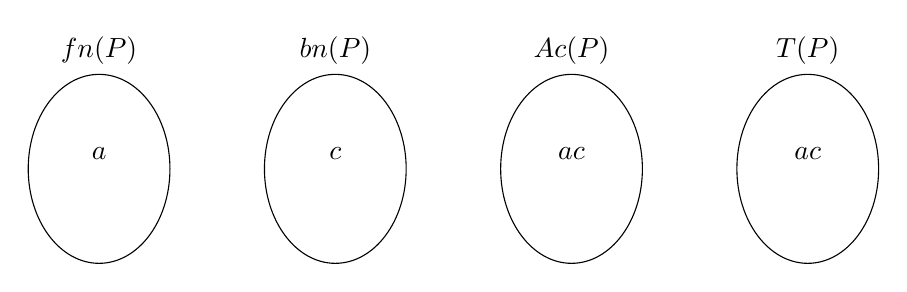
\begin{tikzpicture}
    % draw the sets
   \draw[] (-7.5,0) ellipse [x radius = 0.9cm, y radius = 1.2cm];
    \draw[] (-4.5,0) ellipse [x radius = 0.9cm, y radius = 1.2cm];
    \draw[] (-1.5,0) ellipse [x radius = 0.9cm, y radius = 1.2cm];
    \draw[] (1.5,0) ellipse [x radius = 0.9cm, y radius = 1.2cm];
    % the texts
    \node at (-7.5,1.5) {$fn(P)$};
    \node at (-4.5,1.5) {$bn(P)$};
    \node at (-1.5,1.5) {$Ac(P)$};
    \node at (1.5,1.5) {$T(P)$};

    \node (x1) at (-7.5,0.2) {$a$};

    \node (y1) at (-4.5,0.2) {$c$};

    \node (z1) at (-1.5,0.2) {$\bout{a}{c}$};
    
    \node (w1) at (1.5,0.2) {$\bout{a}{c}$};
\end{tikzpicture}
\caption{traces}
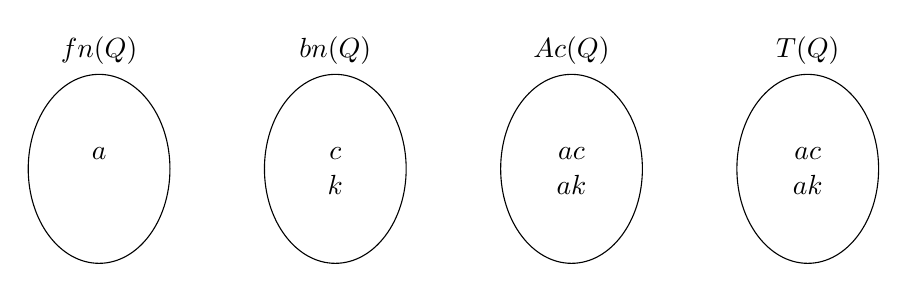
\begin{tikzpicture}
    % draw the sets
    \draw[] (-7.5,0) ellipse [x radius = 0.9cm, y radius = 1.2cm];
    \draw[] (-4.5,0) ellipse [x radius = 0.9cm, y radius = 1.2cm];
    \draw[] (-1.5,0) ellipse [x radius = 0.9cm, y radius = 1.2cm];
    \draw[] (1.5,0) ellipse [x radius = 0.9cm, y radius = 1.2cm];
    % the texts
    \node at (-7.5,1.5) {$fn(Q)$};
    \node at (-4.5,1.5) {$bn(Q)$};
    \node at (-1.5,1.5) {$Ac(Q)$};
    \node at (1.5,1.5) {$T(Q)$};

    \node (x1) at (-7.5,0.2) {$a$};

    \node (y1) at (-4.5,0.2) {$c$};
    \node (y2) at (-4.5,-0.2) {$k$};

    \node (z1) at (-1.5,0.2) {$\bout{a}{c}$};
    \node (z2) at (-1.5,-0.2) {$\bout{a}{k}$};

    \node (w1) at (1.5,0.2) {$\bout{a}{c}$};
    \node (w2) at (1.5,-0.2) {$\bout{a}{k}$};
\end{tikzpicture}
\caption{traces}
\end{figure}